\SetKwProg{Scan}{riboScan}{ }{end}
\SetKwProg{Select}{riboSelect}{ }{end}
\SetKwProg{Seed}{riboSeed}{ }{end}
\begin{figure}[h]
  \centering
  \begin{minipage}{.6\linewidth}
    \begin{algorithm}[H]
      \Seed{(reference, riboSelect\_clusters, reads, iters, flanking\_width)}{
        ref = reference\;
        clusters = parse riboSelect\_clusters\;
        region = clusters + flanking\_width\;
        \For{i in iters}{
          map reads to ref\;
          \For{cluster in clusters}{
            filter and extract reads region\;
            subassemble\;
            return pseudocontig\;
          }
          assess subassembly\;
          \If {success}{
            make pseudogenome from pseudocontigs \;
            ref = pseudogenome \;
          }
        }
        run assembler with reads and pseudocontigs\;
      }
    \end{algorithm}
  \end{minipage}
  \caption{Pseudocode of riboSeed algorithm}
  \label{fig:algo}
\end{figure}
%%%%%%%%%%%%%%%%%%%%%%%%%%%%%%%%%%%%%%%%%%%%%%%%%%%% 5


\begin{figure}[H]
  \centering
  \hspace*{0cm}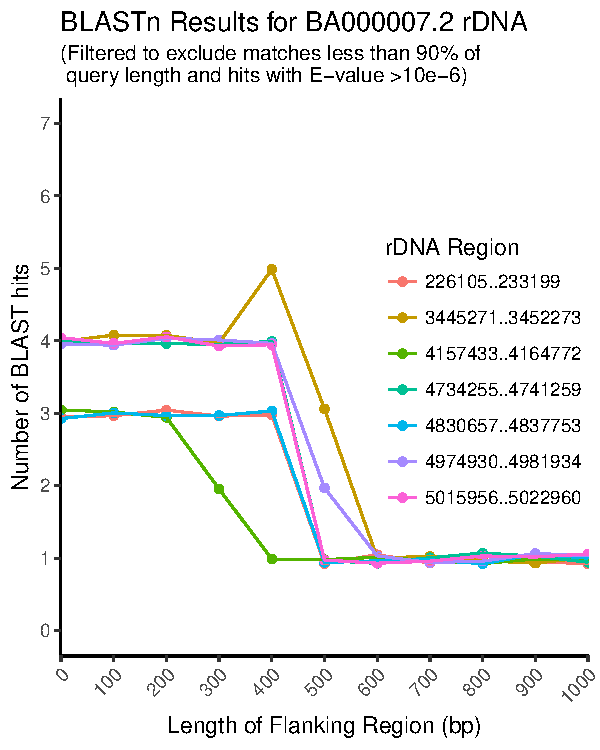
\includegraphics[width=.5\textwidth]{grouped_sakai_BLAST_results}
  \caption{BLASTn was used to perform \textit{in silico} DNA-DNA hybridization of all rDNA regions from \textit{E. coli Sakai} with variable flanking lengths. The number of hits is a proxy for occurrences in the genome; increasing the flanking length increases the specificity. (Points are jittered to aid visibility for overlapping values.)}
  \label{fig:blast}
\end{figure}

\begin{figure}[H]
    \centering
    \hspace*{0cm}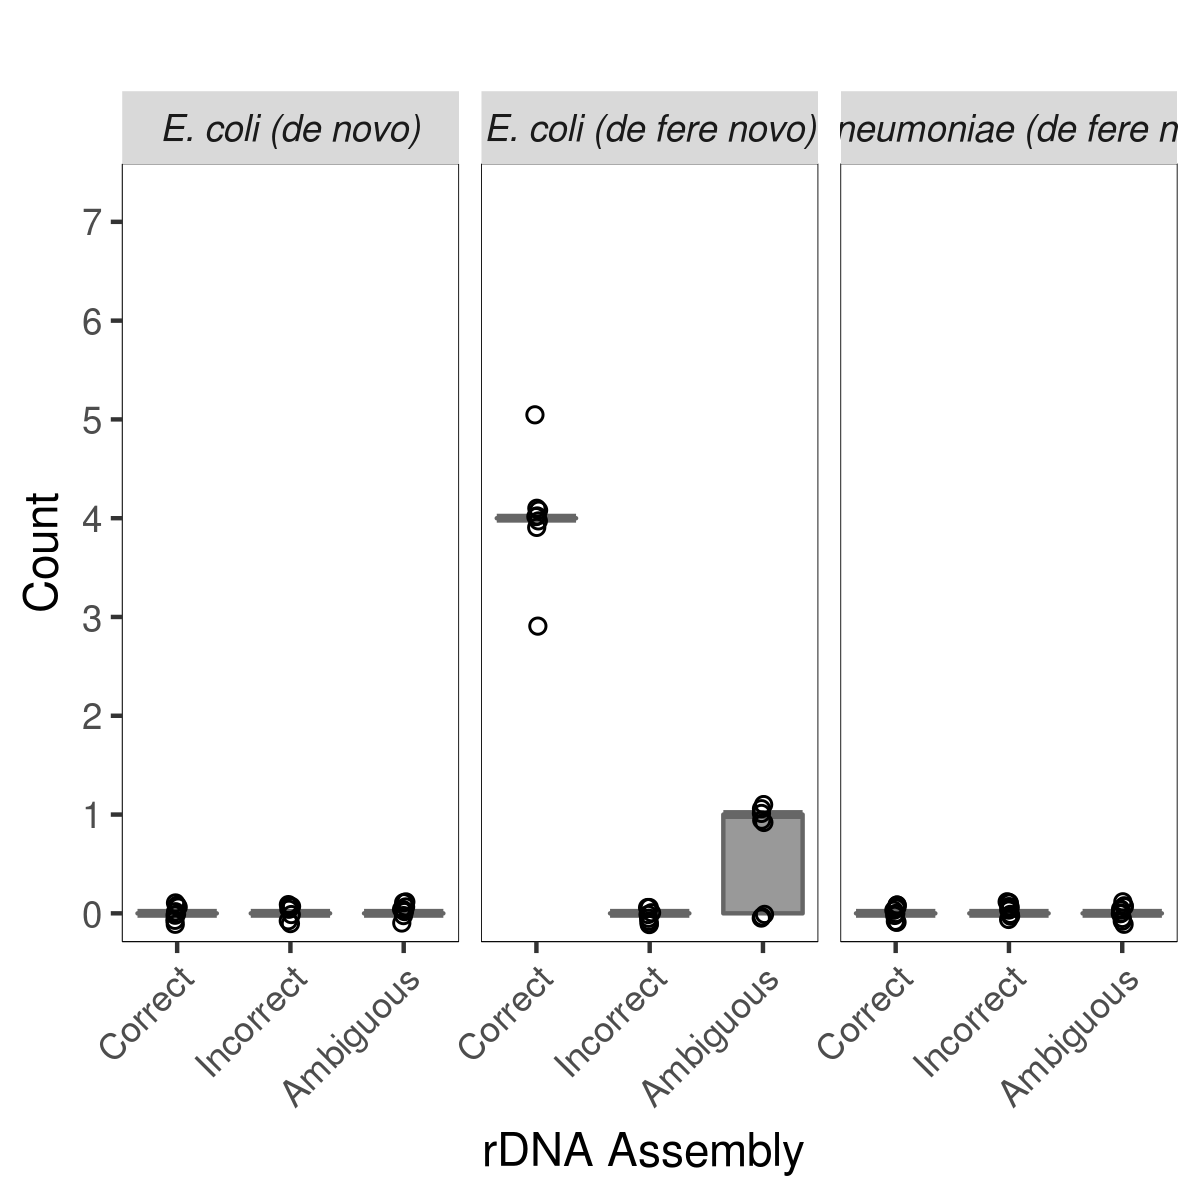
\includegraphics[width=.60\textwidth]{simulated_genome}
    \caption{Assembly of artificial genome. \textit{De fere novo} results in closure of 3-5 rDNAs with the correct reference; only 1-2 rDNAs are correctly assembled using \textit{K. pneumoniae}.  No rDNAs are assembled with \textit{de novo} assembly. Scored with riboScore.py. N=8.}
    \label{fig:simgenome}
\end{figure}



\begin{figure}[H]
  \centering

  \foreach \x in {1,2,...,22}
  {

    \begin{subfigure}[b]{.45\textwidth}
      \includegraphics[width=0.95\textwidth]{entropy_results_figs/\x_genome.png}
      % \caption{\textit{E. coli MG1655} (NC\_000913.3)}
      % \label{fig:ent_coli}
    \end{subfigure}
    \begin{subfigure}[b]{.45\textwidth}
      \includegraphics[width=0.95\textwidth]{entropy_results_figs/\x_gene.png}
      % \caption{\textit{K. pneumoniae subsp. pneumoniae HS11286} (CP003200.1) }
      % \label{fig:ent_pneumo}
    \end{subfigure}
  }
  \caption{riboScan.py,riboSelect.py, and riboSnag.py were run on all the genomes used as references for \textit{de fere novo} assemblies. Consensus alignment depth (grey bars) and Shannon entropy (black points, smoothed entropy as red line) for aligned rDNA regions.  Similar to Figure 3 in the main text, for each genome, a gene neighboring the first rDNA operon was identified, and used to extract homologous rDNA operons from up to 25 other isolates at the species level. In most cases, the entropy is lower in homologous rDNAs than across all the rDNAs in a given genome.}
  \label{fig:ent_gage}
\end{figure}
